\documentclass{article}
\usepackage[utf8]{inputenc}
\usepackage{graphicx}
\usepackage{dirtytalk}
\usepackage{caratula}
\usepackage{amssymb}
\usepackage{amsmath}
\usepackage{geometry}
\usepackage{fixltx2e}
\usepackage{cite}
\geometry{
 a4paper,
 total={210mm,297mm},
 left=30mm,
 right=30mm,
 top=30mm,
 bottom=30mm,
 }
\begin{document}
% Estos comandos deben ir antes del \maketitle
\materia{Métodos Numéricos} % obligatorio

\titulo{Trabajo Práctico 3} % obligatorio
\subtitulo{Si nos organizamos recuperamos rápido...} % opcional
\grupo{     
\\
}
\integrante{Bayardo Julián}{850/13}{julian@bayardo.com.ar} % obligatorio
\integrante{Carrasco Manuel}{646/13}{mgcarrasco2012@gmail.com} % obligatorio 
\integrante{Cuneo Christian}{755/13}{chriscuneo93@gmail.com} % obligatorio 
\integrante{Gómez Fabián}{799/13}{fabiandagomez@hotmail.com} % obligatorio 
\integrante{Keegan Maureen}{761/13}{maukeegan@hotmail.com} % obligatorio 
 
\maketitle

\pagebreak
%\newpage

\section{Introducción Teórica}

Sea una función $F: \mathbb{R} \to \mathbb{R}$ desconocida, y un conjunto de datos $D = \{(x_0, F(x_0)), ..., (x_{n-1}, F(x_{n-1}))\} \subset \mathbb{R}^2$. Supongamos que precisamos interpolar a $F$ por una función $f: [x_0, x_{n-1}] \to \mathbb{R}$. Concretamente, buscamos que $f(x_i) = F(x_i) \forall i \in \{0, .., n-1\}$; además, buscamos que $f$ de alguna forma logre generalizar bien, que logre parecerse a $F$ inclusive cuando la evaluemos en nuevos puntos que no estén en $D$. En la teórica vimos varios métodos para poder encontrar esta $f$ de forma tal que cumpla distintas propiedades según la metodología, pero en este trabajo nos limitaremos a utilizar dos de las vistas: la interpolación lineal, y la interpolación por splines.

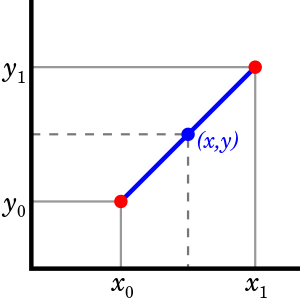
\includegraphics{LinearInterpolation.png}

El primero de estos métodos, la interpolación lineal, consiste en ampliar la clásica idea de buscar una recta que interpole a dos puntos: supongamos que tenemos dos puntos $\{(x_0, y_0), (x_1, y_1)\}$, entonces, y si suponemos que la relación entre ellos es $y(x) = mx + b$, podemos encontrar $m = \frac{y_1 - y_0}{x_1 - x_0}$ y $b = y_0 - m x_0$ como la única recta que pasa por ambos puntos. Supongamos, entonces, que tenemos nuestro conjunto $D$ descripto anteriormente, y tomamos la función

$$f(x) = \sum_{i=0}^{n-2} g_{x_i, x_{i+1}}(x) I_\[x_i, x_{i+1}\)(x)$$

Donde tenemos a $g$ como la función que evalúa a $x$ en la recta que interpola a $x_i$ con $x_{i+1}$:

$$g_{x_i, x_{i+1}}(x) = \frac{F(x_{i+1}) - F(x_i)}{x_{i+1} - x_i} (x - x_i) + y_i$$

Y a $I$ como la función indicadora, que dado un conjunto $A$:

$$I_C(x) =
    \begin{cases}
        1 & \quad \iff x \in A\\
        0 & \quad \text{caso contrario}
    \end{cases}$$
    
Observemos que la función $f$ descripta toma el valor de la recta que interpola a $x_i$ con $x_{i+1}$ en los puntos que pertenecen al intervalo correspondiente. A modo de ejemplo, si tomásemos $F(x) = sin(x)$ con un cierto conjunto de datos $D$, tendríamos una $f$ de la forma:

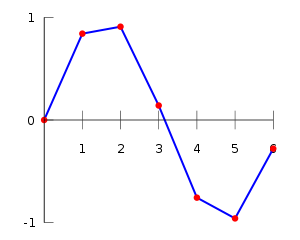
\includegraphics{LinearInterpolationSine.png}

Observemos, además, que cuantos más puntos tengamos, mejor va a ser la aproximación a la función final $F$

\section{Desarrollo}

$\ $ $\ $ $\ $ $\ $Implementamos tres métodos para hacer "zoom" de imágenes: vecino más cercano, interpolación bilineal, e interpolación por splines. En principio, el programa toma por parámetro una imagen en escala de grises $A \in \mathbb{Z}_{256}^{m \times n}$ y un factor $k \in \mathbb{N}_{>0}$ que indica cuánto extenderemos la imagen; concretamente, definimos una familia de transformaciones $f_k : \mathbb{Z}_{256}^{m \times n} \to \mathbb{Z}_{256}^{(k+1)(m-1)+1 \times (k+1)(n-1)+1}$ tal que:

$$(f_k(A))_{i, j} =
    \begin{cases}
        A_{\frac{i - 1}{k + 1} + 1, \frac{j - 1}{k + 1} + 1} & \quad \iff i \equiv 2 (\text{mod} k+1) \wedge j \equiv 2 (\text{mod} k+1) \\
        g_k(A, i, j) & \quad \text{caso contrario}
    \end{cases}$$

Donde $g_k$ es una transformación dependiente del método de interpolación que utilicemos. En concreto, el algoritmo consiste en aplicar la transformación $f_k$ con distintas $g_k$. Para que esta transformación realmente resulte en el efecto visual deseado, queda claro que precisamos de requerimientos muy específicos en términos de qué debería hacer la transformación; a modo de ejemplo, una transformación $g_k(A, i, j) = 0$ nos dejaría una imagen negra en todos los píxeles que no fueran los originales escalados. Para el efecto de agrandar la imagen en particular, queda claro que necesitamos de alguna forma que los píxeles determinados por $g_k$ tengan un sentido estético bien definido: que logren dar una continuidad a los objetos, a fines de que parezcan más grandes. La idea es que al interpolar los píxeles de la imagen real, podemos dar este efecto de continuidad en la nueva imagen.

En el primer método, la idea es que dado un píxel para el que queremos determinar su valor, los píxeles adyacentes en la imagen deberían proveer una buena aproximación al valor que debería tener el píxel realmente. En concreto, el algoritmo se fija cuál es el color del píxel más cercano al que estamos intentando determinar, y pone como valor el resultado de esta comparación. Observemos que podríamos encontrar casos en los que hayan múltiples píxeles a la misma distancia, por lo que debemos determinar cuál de estos valores tomar. En este caso, optamos por tomar la intensidad que se produzca con mayor frecuencia: notemos que $256 = 16 * 16$, es decir, podríamos dividir las posibles intensidades en 16 intervalos de 16 elementos (del 0 al 15, del 16 al 32, etcétera); por lo tanto, en el caso en que tengamos que hay más de un píxel a la misma distancia del punto central, podríamos tomar el punto cuyo intervalo correspondiente es el más frecuente. De cualquier forma, observemos que este criterio también podría fallar, en este caso, optamos por simplemente elegir el primer vecino más cercano descubierto.

En concreto, esperamos que este algoritmo genere imágenes que tiendan a mantener niveles similares de intensidad: los primeros dos criterios de alguna forma nos garantizan dos cuestiones: la primera, que vamos a mantener la intensidad muy fuertemente de forma local, ya que el hecho de elegir vecinos nos garantiza que todos los píxeles en la imagen final van a ser "parecidos"; la segunda, que los niveles de intensidad se van a mantener a nivel global, ya que vamos a tender a replicar los intervalos de mayor frecuencia en la imagen.

El segundo método, la interpolación bilineal, es ligeramente más complicado que el anterior: consiste en elegir una $g_k$ que nos permita hacer dos rondas de interpolaciones. La primera etapa consiste en interpolar dentro de cada una de las filas a los píxeles de la imagen original; observemos que si tomamos el índice $j$ en una de las filas, y el índice $l = j + 1$, ambos mapean en la nueva imagen de forma tal que están separados por $k$ píxeles: si entonces tomamos a $j'$ y a $l'$ como los índices anteriores en la nueva imagen, podemos encontrar una recta que pase por los valores $(j', A_{i, j})$ y $(l', A_{i, l})$. Nótese que esta recta posee dos propiedades interesantes: en primer lugar, todos los índices naturales entre $j'$ y $l'$ pertenecen al dominio; en segundo lugar, la imagen de la recta toma valores que interpolan a los valores de la matriz original, por lo que intuitivamente estamos generando un degradé de la intensidad de la imagen, convirtiendo la intensidad de un punto en la intensidad de otro. 

Habiendo encontrado esta recta, podemos determinar la intensidad de los píxeles en la fila $i$, de las columnas $j'$ a $l'$ como los valores de la recta interpoladora redondeados a enteros. Repetir este proceso para todos los valores de $j$ hasta el $n - 1$, y para todos los valores de $i$ nos crearía una imagen con todas las filas que ya estaban en la imagen original llenas de valores de intensidad, y tan sólo faltaría completar las $k$ columnas vacías que se generan entre cada fila. Pero observemos que podemos llevar a cabo este mismo proceso entre cada una de las columnas, generando la imagen completa.

Es fácil darse cuenta que la imagen nueva mantendrá los niveles de luminosidad de la imagen inicial, ya que todo el tiempo estaremos interpolando por rectas, que no nos permitirán salirnos de rango y terminar saturando los valores. Además, sería esperable que obtengamos mayores discrepancias en las columnas completamente agregadas por el método de interpolación (en el ejemplo, las columnas con índices entre $j'$ y $l'$), ya que estas habrán sido creadas enteramente a través de aproximaciones lineales. Conjeturamos, también, que probablemente este método introduzca un menor error que el primero, ya que el primer algoritmo probablemente genere una idea de discontinuidad en la frontera del radio afectado por un píxel: eventualmente se debe pasar de un vecino a otro, y ese efecto no coincide con la experiencia sensorial, que da más una sensación de suavidad entre los colores. A pesar de esto, estimamos que este método va a tener problemas en términos más globales, ya que un degradé no necesariamente es la forma en la que los objetos se encuentran delimitados en la vida real; a modo de ejemplo, imaginemos un escritorio de madera con una pared blanca de fondo: los bordes del escritorio van a tener una transición de color abrupta, una especie de discontinuidad, mientras que las partes íntegramente de madera van a tener una transición más suave, o de degradé entre los valores de luminosidad.

El tercer método, la interpolación por splines, consiste en aumentar la complejidad del método anterior: en lugar de considerar interpolaciones lineales entre dos píxeles, tomamos polinomios de grado 3 que interpolen un conjunto de píxeles. El sentido está en pedir que estos polinomios cumplan una serie de características de spline, que nos permitirán afirmar no sólo que interpolan a los puntos requeridos, sino que además preservan la idea de continuidad de la intensidad. Más aun, al ser polinomios que tomen tanta información en cuenta, también harán una mejor transición en los bordes de los objetos, que nos garantiza una mejoría con respecto a la interpolación lineal del método anterior.

\pagebreak

\section*{Desarrollo}{}
\end{document}